\section{Berechnung der Dense Units}
<<<<<<< HEAD
\label{sec:chap3}

=======
Clusters von benachbarten Punkten müssen zu einem minPoint Großen subsets kombiniert werden. Diese subsets werden Dense Units genannt.
>>>>>>> 4e4bcdda93ef5b884d3aa359162611458d088d35
Dense Units werden in verschiedene Funktionen mit unterschiedlichen Zwecken berechnet. Das Hauptziel dieser Berechnung, ist die Bestimmung einer Teilmenge aus allen möglichen Kombinationen in einem subset. Dabei dürfen keine Wiederholungen der Dense Units auftreten. Die Kombinationen aus einem subset können mittels dem Binominialkoeffizient berechnen, $ \binom{n}{k} $ dabei ist n die Anzahl der Elemente in dem subset und k die minimale Anzahl an punkten in einem subset (e.g. minPoints). Daraus entstehen k-Elemente großes subsets von einem n-Elemente set ohne Wiederholungen der Kombinationen.
Wenn zum Beispiel ein Core Set aus folgenden Punkten besteht: [1, 5, 7, 9, 22] und die minimale Anzahl an punkten in einem Subset Drei ist, sind die ersten Drei Dense Units folgende: [1, 5, 7] und [1, 5, 9] und [1, 5, 22]. Die Formel zur Berechnung der Dense Units kann also folgendermaßen betrachtet werden: 
$ \binom{|CS|}{minPoints}$ \cite{7022654} Abbildung \ref{dense-calculation} zeigt ein weiteres Beispiel für n-Punkte in einem Core Set mit minPoints von 4.

\begin{figure}
	\centering
	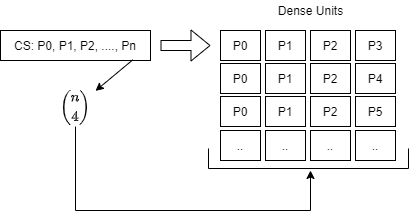
\includegraphics[width=0.5\textwidth]{DenseUnitBerechnung.png}
	\caption{Berechnung der Dense Units}
	\label{dense-calculation}
\end{figure}